\section{Przeprowadzone testy}

\subsection{Test poprawności trasowania}

\begin{figure}[H]
	\centering
	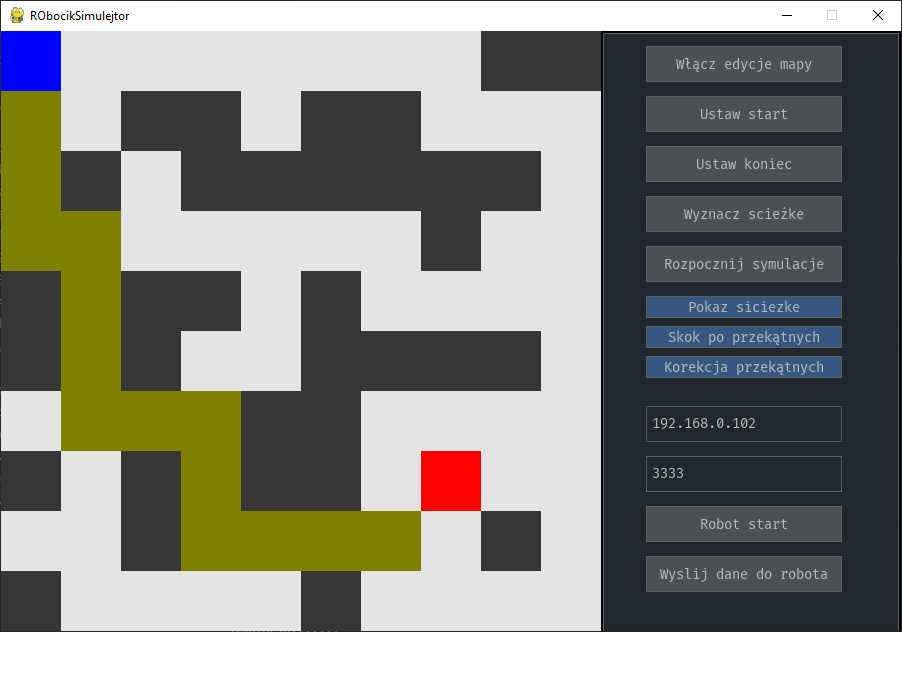
\includegraphics[width=13cm]{pages/testy/zdjecia/t1_1.png}
	\caption{Podstawowy test trasowania}
	\label{Fig:schematSerweraTCP}
\end{figure}




\subsection{Wpływ ustawień na wyznaczoną ścieżkę}

\begin{figure}[H]
	\centering
	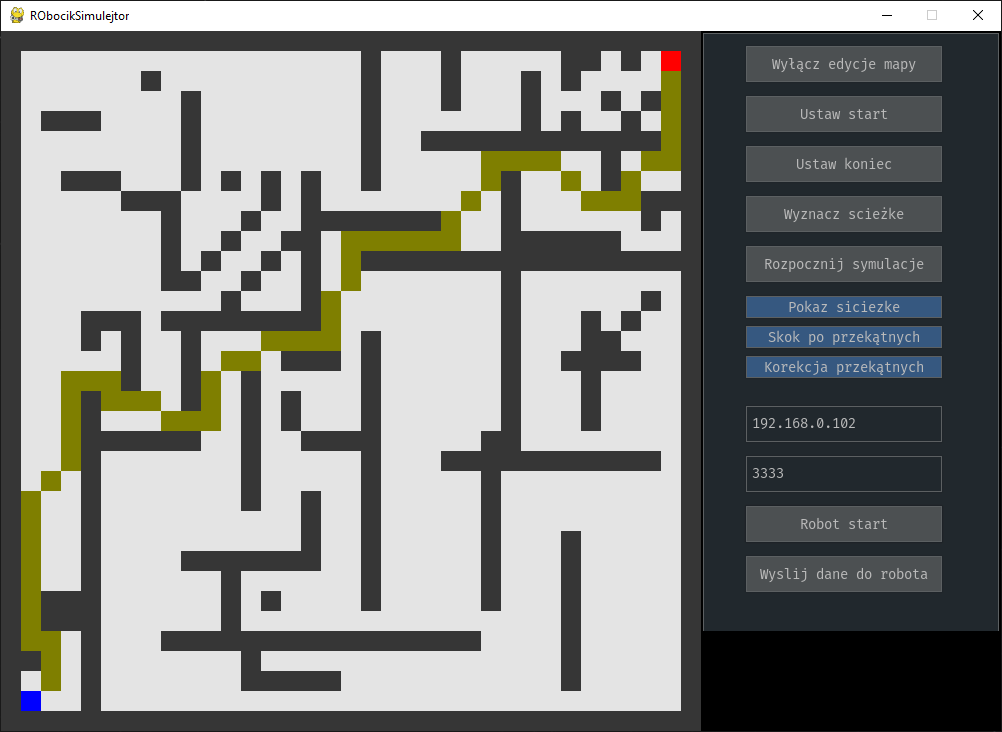
\includegraphics[width=13cm]{pages/testy/zdjecia/t2_1.png}
	\caption{Wyznaczona ścieżka, włączona korekcja i przejście po przekątnej}
	\label{Fig:test21}
\end{figure}


\begin{figure}[H]
	\centering
	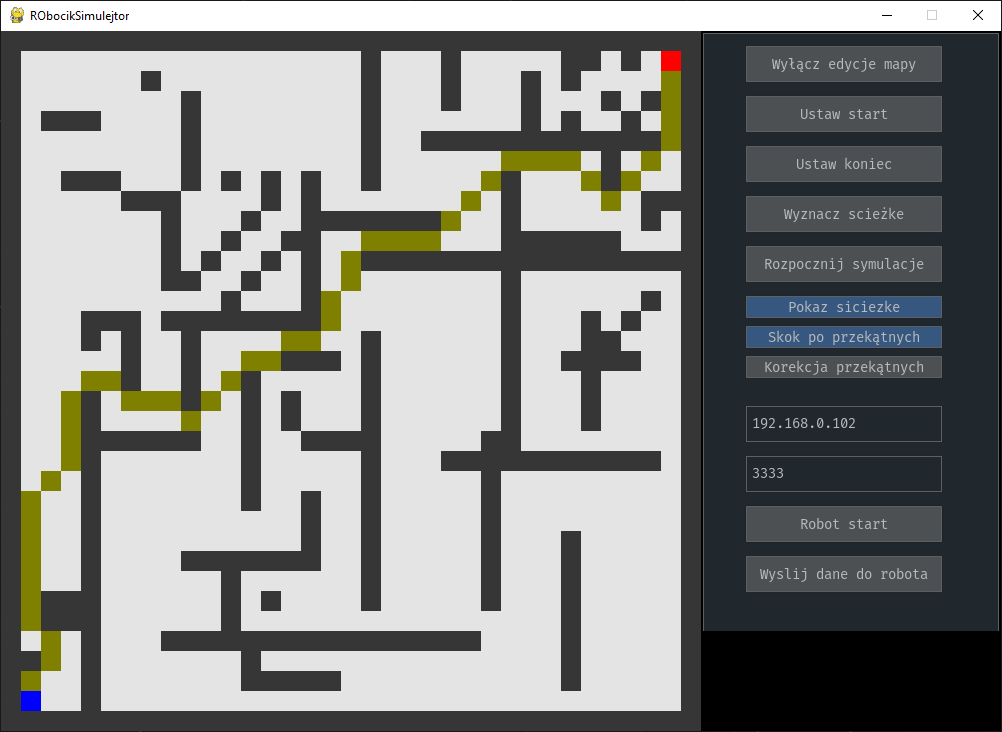
\includegraphics[width=13cm]{pages/testy/zdjecia/t2_2.png}
	\caption{Wyznaczona ścieżka, korekcja przekątnych jest wyłączona}
	\label{Fig:schematSerweraTCP}
\end{figure}


\begin{figure}[H]
	\centering
	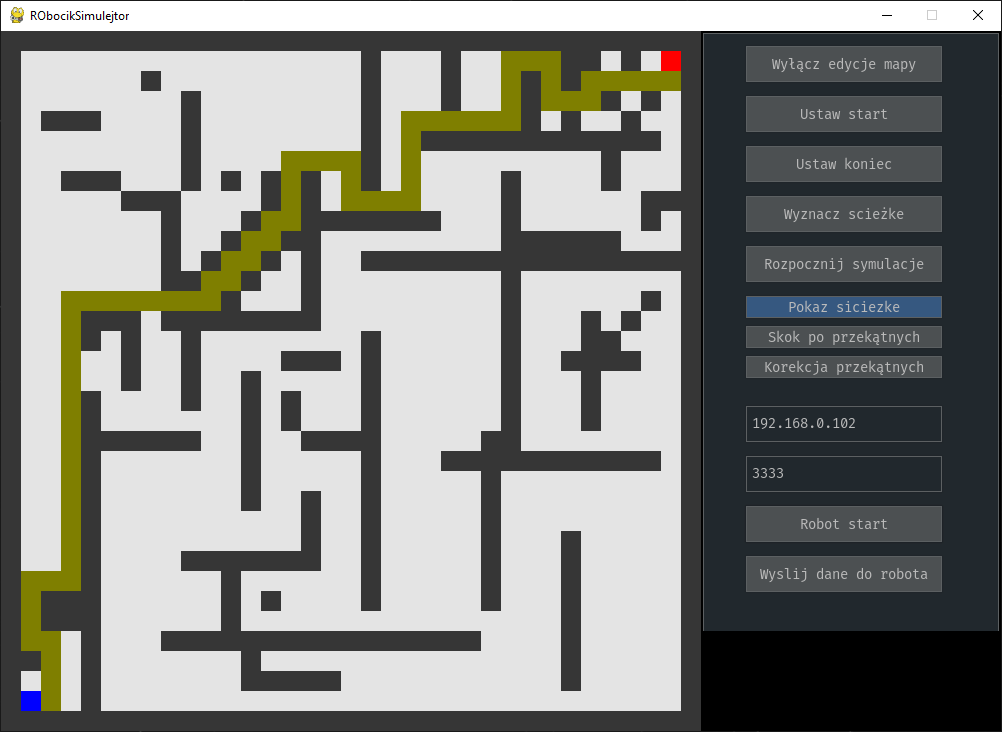
\includegraphics[width=13cm]{pages/testy/zdjecia/t2_3.png}
	\caption{Najkrótsza trasa, wyłączone przejście po przekątnych}
	\label{Fig:schematSerweraTCP}
\end{figure}

\subsection{Sprawdzenie wpływu funkcji heurestycznej na ścieżkę}

\subsection{Test komunikacji z fizycznym robotem}

